\documentclass[12pt]{article}
\usepackage{verbatim}
\usepackage[dvips]{epsfig}
\usepackage{color}
\usepackage{url}
\usepackage[colorlinks=true]{hyperref}

\begin{document}

\section*{GENESIS: Documentation}

{\bf Related Documentation:}
% start: userdocs-tag-replace-items related-do-nothing
% end: userdocs-tag-replace-items related-do-nothing

\section*{The GENESIS Graphic User Interface}

\section*{Introduction}

The GENESIS graphic user interface ({\bf G-Tube}) provides an
interactive environment for the construction, modification, and
simulation of computational models of subcellular mechanisms, neurons
and neural circuits.  A demonstration session that runs a simulation
with the G-Tube can be found \href{../gtube-demo/gtube-demo.html}{here}.

{\bf G-Tube} is developed according to the principles of the Computational Biology Initiative Federated Software Architecture which is described in the \href{../genesis-overview/genesis-overview.tex}{\bf GENESIS\,Overview}. The underlying philosophy of the GUI's modular software design is that it follows the \href{../workflow-intro/workflow-intro.tex}{\bf GENESIS\,user\,work\,flow} and supports the work flow's five basic steps:
\begin{enumerate}
\item {\bf Create/import, explore, and save model.}
\item {\bf Define simulation constants, inputs, and outputs.}
\item {\bf Check, run, reset simulation, and save model state.}
\item {\bf Check simulation output.}
\item {\bf Iterate.}
\end{enumerate}
The block diagram given below illustrates the relationships between the software components that support this GUI functionality.

\begin{figure}[h]
  \centering
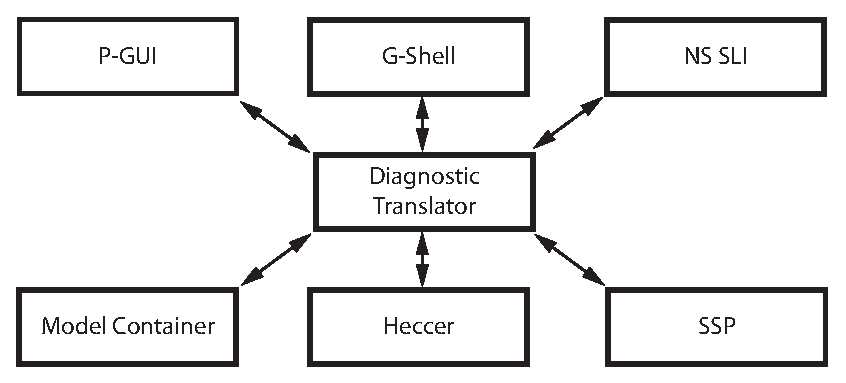
\includegraphics[scale=0.6]{figures/gui-isolated.eps}
%\caption{{\bf GUI software layout:} The GENESIS GUI is illustrated in this software block diagram.}
  \label{fig:df-1}
\end{figure}

\subsection*{User Interface Functions:} {\bf G-Tube} can be initiated from either a \href{../unix-linux/unix-linux.tex}\bf {\bf UNIX\,prompt} or the \href{../gshell/gshell.tex}{\bf G-shell}. Alternatively, There is a GUI that provides backward compatibility with previous versions of GENESIS (Version 2.3 and earlier).

\begin{itemize}
   \item {\bf P-GUI:} This refers to the initiation of the Python/Perl enabled {\bf G-Tube} from the command line of a terminal window.
   \item {\bf G-shell:} The same GUI can also be initiated from the G-shell.
   \item {\bf NS-SLI:} This refers to the Neurospaces Script Language Interpreter that provides backward compatibility with the Script Language Interpreter of earlier versions of GENESIS.
\end{itemize}

The Diagnostic Translator is a middle ware software component that enables interaction between the user (via a given GUI component--{\bf G-Tube}, {\bf G-Shell}, or {\bf NS-SLI}) and the \href{../model-container/model-container.tex}{\bf Model\,Container}, \href{../heccer/heccer.tex}{\bf Heccer}, or \href{../ssp/ssp.tex}{\bf SSP}.

\section*{G-Tube Installation}

{\bf G-Tube} is a GUI implemented in Python which simplifies the use of GENESIS. It is currently under development so functionality is limited. Bugs and feature requests should be reported to the authors to ensure users are satisfied with the end result.
Details

\section*{G-Tube Developer Repository}

{\bf G-Tube} is verisoned in \href{http://mercurial.selenic.com/}{\bf mercurial} and has a repository served over the internet to show the status of the latest checkins at the following website. \href{http://repo-genesis3.cbi.utsa.edu/hg/g-tube/}{\bf http://repo-genesis3.cbi.utsa.edu/hg/g-tube/}


\subsection*{Dependencies}

To install {\bf G-Tube} you need the following packages installed on your machine.

\begin{itemize}
   \item {\href{http://python.org/download/}{\bf Python 2.5:}} You can check the version you have installed with
   
   ``{\tt python -V}''
   
   \item {\bf wxPython:} Version 2.8 or higher from:   
   \begin{itemize}
      \item \href{http://www.wxpython.org/download.php}{\bf wxPython site}
      \item Direct link to \href{https://sourceforge.net/projects/wxpython/files/}{\bf Sourceforge}
   \end{itemize}
   \item \href{http://pyyaml.org/ }{\bf PyYAML}:
\end{itemize}

\subsection*{Building wxPython from source}

To use wxPython you must first build wxWidgets, which is included with the wxPython source tarball. To build wxWidgets you'll need the following libraries installed. To compile you'll need {\it g++}.

\begin{itemize}
   \item {\it zlib-dev}
   \item {\it libjpeg-dev}
   \item {\it libpng-dev}
   \item {\it libtiff-dev}
   \item {\it libgtk-dev}
\end{itemize}

    If you want 3D bindings you'll need: 

\begin{itemize}
   \item {\it libglut-dev}
\end{itemize}

Once wxWidgets is built be sure to run {\it ldconfig}. After building and setting up wxWidgets go into the wxPython directory and use the Python script {\it setup.py} to build and install the wxPython bindings.

\end{document}
